\chapter{Planification And Architecture}
\newpage
\begin{center}
    \doublespacing 
    \centering
    \LARGE\textbf{Introduction} 
     \vspace{1cm} \\
   \raggedright
\end{center}
\Large As outlined in the previous chapter, we have decided to use the Scrum methodology for the design of our platform.  
In this chapter, titled "Planning and Architecture" or "Sprint Zero," we will undertake the initial phase of the Scrum approach. This involves defining user roles, identifying functional and non-functional requirements, and compiling them into a product backlog.

\section{Requirements Specification}
To successfully achieve the desired goals, it is important to frame the project properly by aligning it with the necessary requirements and a well-thought-out plan.
\subsection{Actors Identification}
\Large Here’s a structured and humanized description of each actor and their role, showing how responsibilities escalate through the hierarchy:   

\subsubsection{Insured}
The insured person is the primary user of the platform. They can: 
\begin{itemize}
    \item  Submit requests through dynamic forms.
    \item  Track the status of their submissions.
    \item  Manage their personal profile.
\end{itemize}
Once they submit a request, it enters the system, where different actors handle and review it.  

\subsubsection{Submission Coordinators}  
This level includes two key roles responsible for processing submissions before they reach higher authorities:  

\textbf{- File Manager:}\\
\begin{itemize}
    \item  Reviews submitted requests to ensure they are complete and accurate.
    \item  If necessary, forwards submissions for further processing.
\end{itemize}

\textbf{- Office Supervisor: } 
\begin{itemize}
    \item  Oversees the submission process within an office.
    \item  Tracks workflows and ensures smooth operations.
    \item  Views office and basic statistics to monitor performance.
\end{itemize}


\subsubsection{ Central Agent} 
\begin{itemize}
    \item  Manages both "File Managers" and "Office Supervisors" to ensure efficient processing.
    \item  Ensures proper coordination and treatment of the files that have been escalated to him.
\end{itemize}

\subsubsection{ Central Manager } 
\begin{itemize}
    \item  Holds the highest authority in the system.
    \item  Publishes important news and updates on the platform.
    \item  Monitors global statistics to track overall performance.
    \item  Ensures system-wide efficiency.
    \item  Authenticates users and ensures security.
\end{itemize}

\subsection{Escalation Flow}  
\begin{enumerate}
    \item Insured submits a request.
    \item Submission Coordinators (File Manager and Office Supervisor) review and process it. If necessary, they escalate to the Central Agent for higher-level management.
    \item The "Central Agent" ensures proper handling.
\end{enumerate}
This hierarchy ensures an organized workflow, with responsibilities clearly defined at each level.
\subsection{Static Context Diagram}
A static context diagram helps determine how the system relates to the actors and establishes how many instances of the different actors exist at one point in time to the system.
\begin{figure}[h]
    \centering
    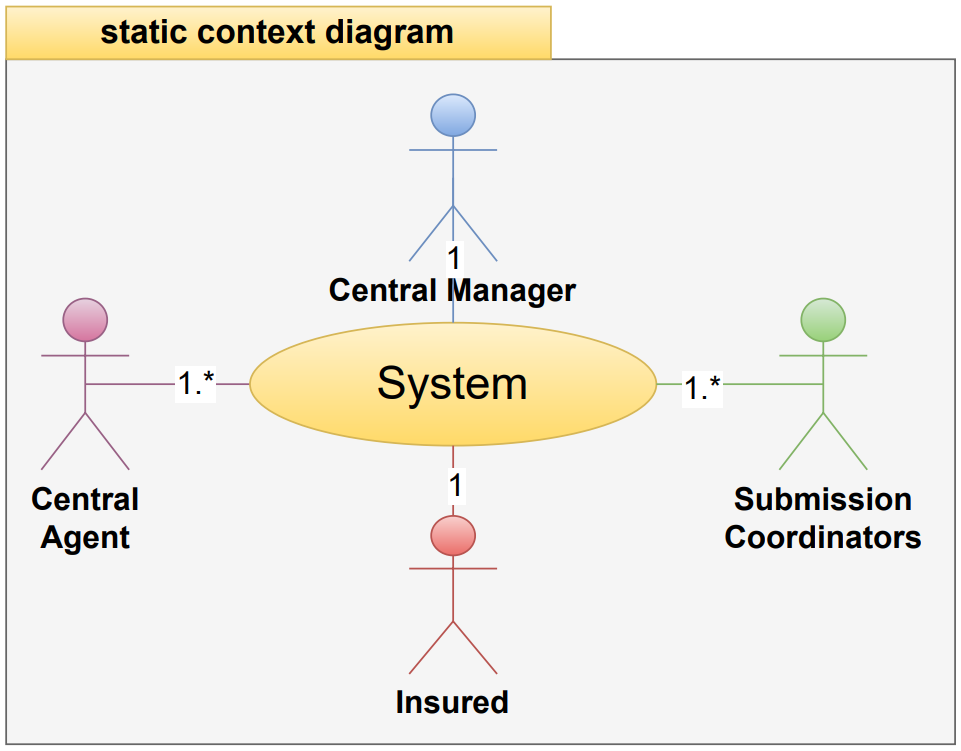
\includegraphics[width=0.6\textwidth]{figures/statdia.png}
    \caption{Static context Diagram.}
\end{figure} \ 
\subsection{Identification of Functional Requirements}
Functional requirements or use cases from the perspective of UML can be described as follows: \textbf{"A use case explains how users interact with a product or system. It outlines the flow of user inputs, establishing successful and failed paths to meeting goals."}\cite{samplewebs4}\\
Functional requirements define the functionalities of the system that are made available to different actors to satisfy their needs and expectations.
Each of the functional requirements is a list of steps executed by our system in order to react to an application's request.
\begin{enumerate}
    \item Insured

     \begin{itemize}
         \item Submit requests through dynamic forms.
         \item Track the status of submissions (e.g., pending, approved, rejected).
         \item View notifications (approvals, rejections).
         \item Alerts for submissions.
         \item Access news/announcements published on the platform.
         \item Manage profile (update personal details).
     \end{itemize}
 
\item File Manager
\begin{itemize}
    \item Review submissions according to his actual region.
    \item Escalate further files to the Office Supervisor + adds additional documents if needed.
    \item Access basic statistics.
\end{itemize}
    
\item Office Supervisor
\begin{itemize}
    \item Review forwarded submissions (from File Managers).
    \item Supervise assigned File managers (review their work).
    \item Escalate to Central Agent  + adds additional documents if needed.
    \item Access basic statistics.
\end{itemize}
    
\item Central Agent
\begin{itemize}
    \item Manage File Managers and Office Supervisors (create accounts, assign roles).
    \item Review submissions forwarded from the Office supervisors.
    \item View basic statistics.
    \item Review the office supervisors work.
\end{itemize}

\item Central Manager
\begin{itemize}
    \item Publish platform news/updates.
    \item Configure dynamic forms (customize fields).
    \item Manage internal stakeholders.
    \item Tracks the flow of every submissions process.
    \item View global statistics.
\end{itemize}
    
\item System (Automated Functions)

\begin{itemize}
    \item Authenticate users (secure login, role-based access).
    \item Send automated emails (notifications, status updates).
    \item Validate national identity documents and extract important data.
    \item Generate automated statistics.
\end{itemize}
\end{enumerate}
\subsection{Identification of Non-Functional Requirements}
At some stage in the project life, the team has to consider non-functional requirements. These are requirements that lie within the system and are invisible to the end-user. The platform has to satisfy the following conditions:

\begin{itemize}
    \item \textbf{Performance:} Also known as response time, is a growing concern. There is a need to optimize our platform's page loading times.

\item \textbf{Accessibility:} Our website is at the core of the Information System Department operations, and therefore it is critical that it is operational at all times.

\item \textbf{Usability:} The interfaces must be easy to use and not complicated by adhering to usability guidelines.
  
\item \textbf{Security:} Since the application is filled with personal information, the access to different parts must be protected through passwords and access privileges.
  
\item \textbf{Maintainability:} The code must be structured in a readable, well-organized, and clear form to facilitate the maintenance of the various modules of the application.
\item \textbf{Storage:} As our platform deals with a huge quantity of non-structured data therefore we insured that the documents are well archived including relevant meta data for easy retrieval and organisation.
\end{itemize}
\section{ Project Structure and Breakdown}
\subsection{Identification of the SCRUM Team}
The most critical stakeholder of SCRUM is the SCRUM team.
In our project example, Mr. Oussama Cherif will be the Product Owner because he meets all the requirements to be a Product Owner. Ms. Saoussen Anssi will be the Scrum Master, and we, Nourchene Garbouj and Yassine Ben Yedder, are the Development Team.
\begin{figure}[h]
    \centering
    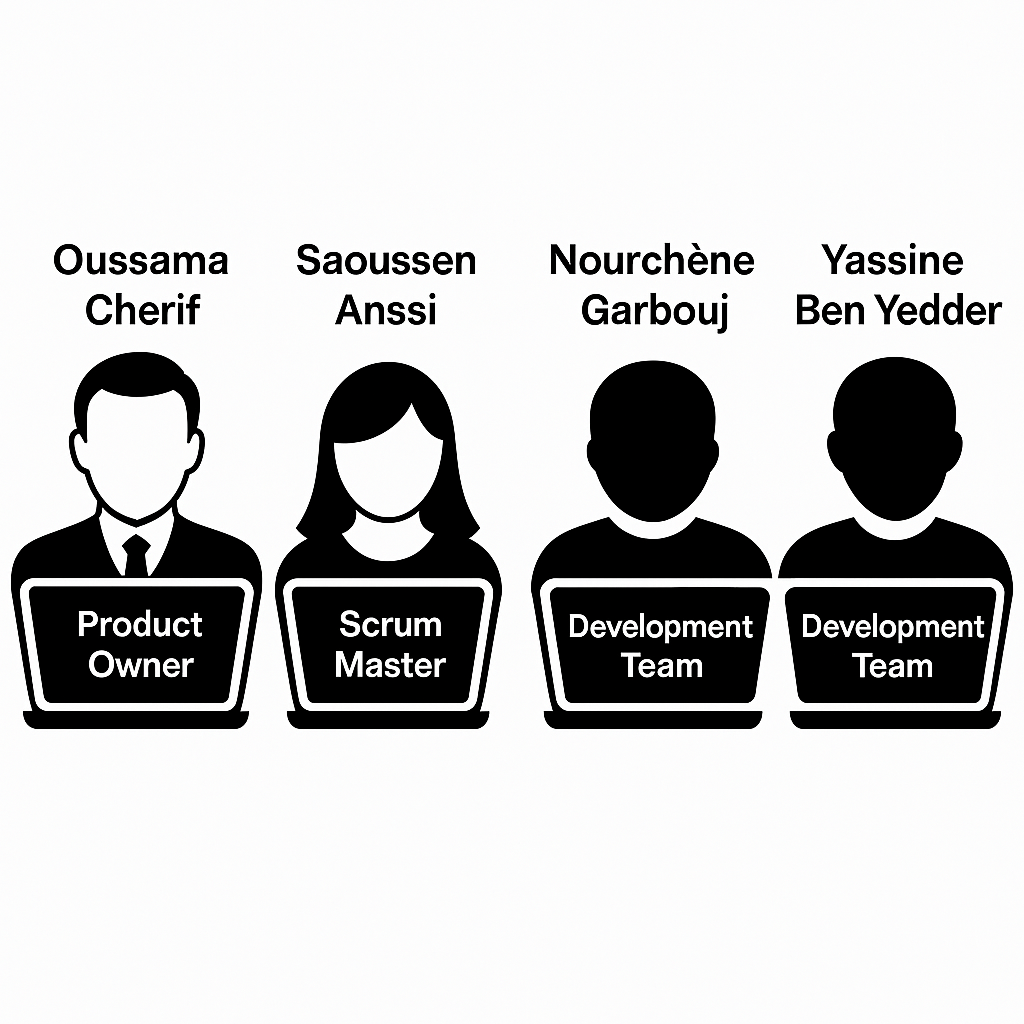
\includegraphics[width=0.7\textwidth]{figures/scrumteam.png} 
    \caption{Roles of the Team.}
\end{figure} \

\subsection{Product Backlog}
As defined in the first chapter, the product backlog is a very important artifact that represents the expected requirements and functionalities.  
We present in Table 2.1 a summary of the product backlog related to our solution, which lists the following fields:

\begin{itemize}
    \item \textbf{ID:} A unique and incremented identifier for each new User Story.
    \item \textbf{User Story:} Describes the content of a functionality.
    \item Description: A short description of the task to be completed, defined as follows: As a <role>, I want to <do something> so that <I can get value>.
    \item \textbf{Priority:} The level of importance assigned to this task by the Product Owner (High or Medium).
    \item S\textbf{tory Points:} are a relative measure of effort used to estimate the complexity, work, and risk of a user story.
\end{itemize}


\newcolumntype{L}[1]{>{\raggedright\arraybackslash}p{#1}}
\begin{longtable}{|c|L{3.5cm}|L{4.4cm}|c|c|}
\hline
\textbf{ID} & \textbf{User Story} & \textbf{Description} & \textbf{Priority} & \textbf{Story Points} \\
\hline
\endfirsthead
\hline

01 & Submit requests via dynamic forms & As an \textbf{Insured}, I want to submit requests through dynamic forms so that my requests can be processed properly. & High & 8 \\
\hline
02 & Validate national ID documents & As a \textbf{System}, I want to validate identity documents so that I can extract reliable user data. & High & 8 \\
\hline
03 & Manage dynamic forms & As a \textbf{Central Manager}, I want to manage dynamic forms so that forms can be customized when needed. & High & 6 \\
\hline
04 & Authenticate & As a \textbf{User}, I want to authenticate so that I can access the platform securely. & High & 5 \\
\hline
05 & Review submission & As a \textbf{Submission Coordinator}, I want to review submissions so that I ensure their correctness. & High & 5 \\
\hline
06 & Review forwarded submissions & As a \textbf{Central Agent}, I want to review forwarded submissions so that I can validate them centrally. & High & 5 \\
\hline
07 & Manage user roles & As a \textbf{Central Agent}, I want to manage File Managers and Office Supervisors so that I ensure proper workflow. & High & 5 \\
\hline
08 & Track submission workflows & As a \textbf{Central Manager}, I want to track workflows so that I can monitor overall submission health. & High & 6 \\
\hline
09 & Reset forgotten password & As an \textbf{Insured}, I want to reset my password so that I can regain access to my account. & High & 3 \\
\hline
10 & Track submission status & As an \textbf{Insured}, I want to track the status of my requests so that I stay informed about their progress. & Medium & 5 \\
\hline
11 & Manage profile & As a \textbf{User}, I want to manage my profile so that my personal information stays up to date. & Medium & 3 \\
\hline
12 & View basic statistics & As a \textbf{Submission Coordinator}, I want to view basic statistics so that I can analyze performance. & Medium & 3 \\
\hline
13 & Consult notifications & As an \textbf{Insured}, I want to consult notifications so that I don’t miss important updates. & Medium & 3 \\
\hline
14 & Monitor office supervisors & As a \textbf{Central Agent}, I want to monitor office supervisors so that I ensure their tasks are progressing. & Medium & 4 \\
\hline
15 & Monitor file managers & As an \textbf{Office Supervisor}, I want to monitor file managers so that I can supervise their work. & Medium & 4 \\
\hline
16 & View global statistics & As a \textbf{Central Manager}, I want to view global statistics so that I can evaluate platform performance. & Medium & 4 \\
\hline
17 & Manage internal stakeholders & As a \textbf{Central Manager}, I want to manage stakeholders so that I can ensure project alignment. & Medium & 5 \\
\hline
18 & Receive submission emails & As an \textbf{Insured}, I want to receive email notifications so that I am alerted about any updates on my submissions. & Medium & 2 \\
\hline
19 & See platform news & As an \textbf{Insured}, I want to see the news so that I stay informed about platform announcements. & Medium & 2 \\
\hline
20 & Publish news & As a \textbf{Central Manager}, I want to publish news on the platform so that users are informed. & Medium & 2 \\
\hline
\caption{Product Backlog Table}
\end{longtable}

\subsection{SCRUM Tool}
Jira is a powerful project management tool designed to support Agile and Scrum methodologies. It allows teams to plan and manage sprints, track tasks through customizable boards, and organize product backlogs efficiently. With features like real-time collaboration, workflow automation, and detailed reporting, Jira enhances team visibility and productivity. It also supports Scrum ceremonies such as sprint planning, reviews, and retrospectives, promoting continuous improvement throughout the development cycle.
\begin{figure}[h]
    \centering
    
\includegraphics[width=0.6\textwidth]{figures/jira logo.png} 
    \caption{Roles of the Team.}
\end{figure} \

\subsection{Sprint Structure}
\subsubsection{Project Sprint Planning}
The sprint planning phase is vital to the successful execution of a project. It provides for the best approach to task decomposition and allocation based on priorities, time, and team capacity, in order to be able to meet the requirements laid out by the Product Owner better.\\
\textbf{"Sprints are time-constrained periods of one week to one month, during which a product owner, Scrum master and Scrum team work to complete a specific product addition. During a sprint, work is done to create new features based on the user stories and backlog."}\cite{samplewebs5}
\begin{figure}[h]
    \centering
    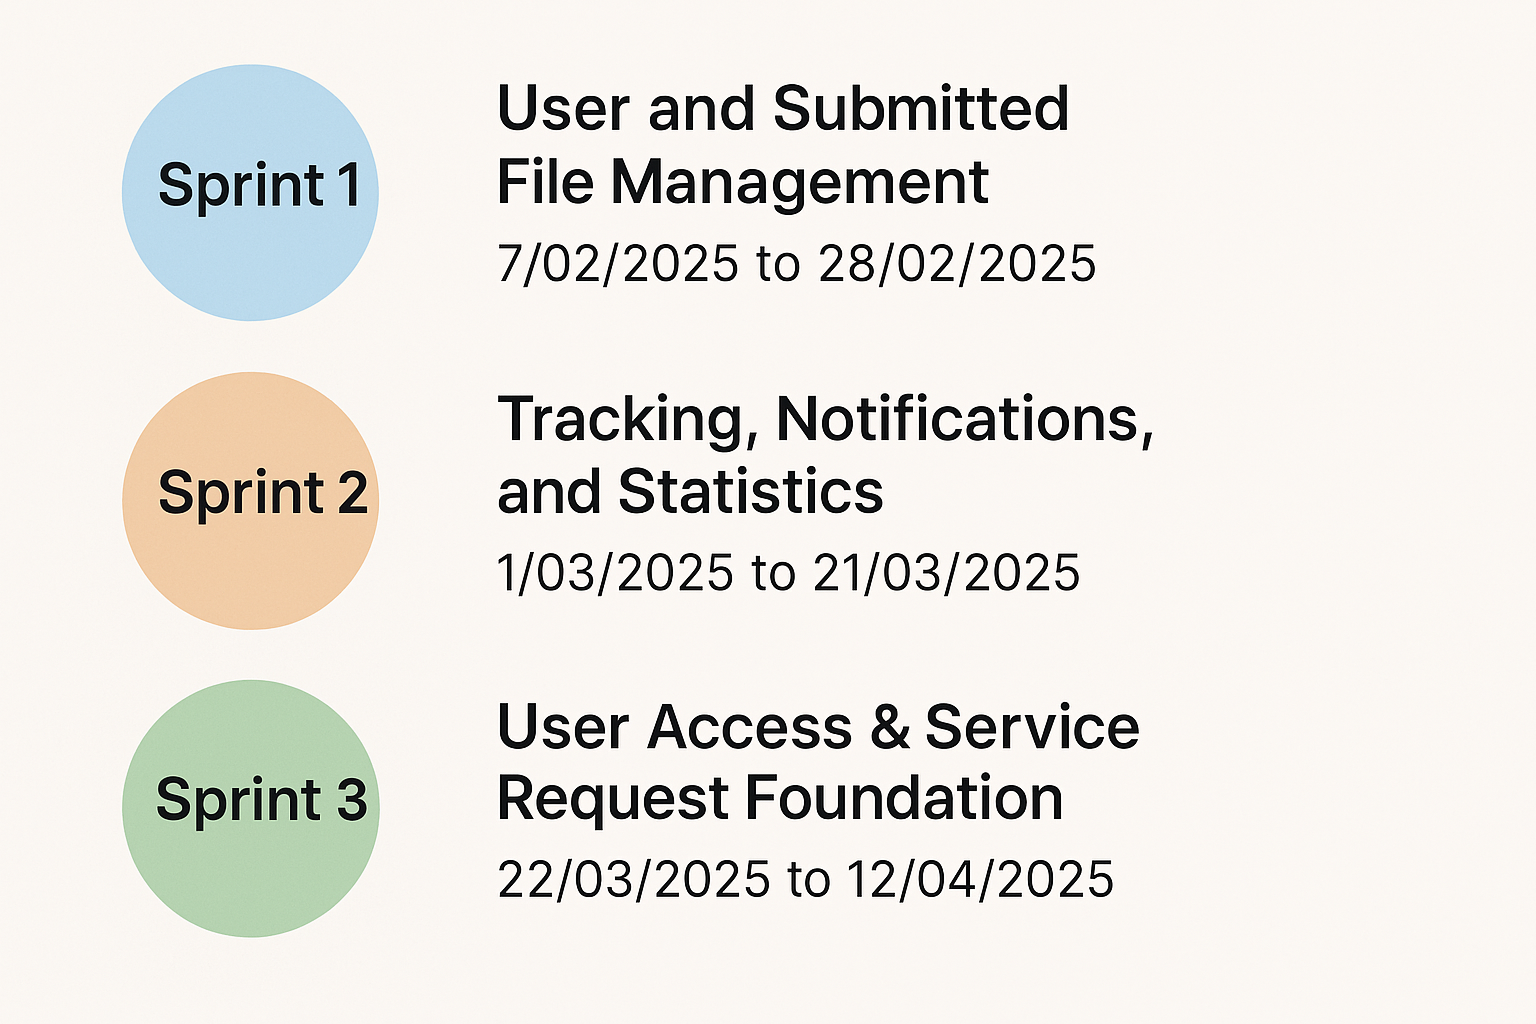
\includegraphics[width=0.5\textwidth]{figures/sprints.png}  
    \caption{Sprints Planification.}
\end{figure} \
\subsection{Project execution plan}
\begin{figure}[h]
    \centering
    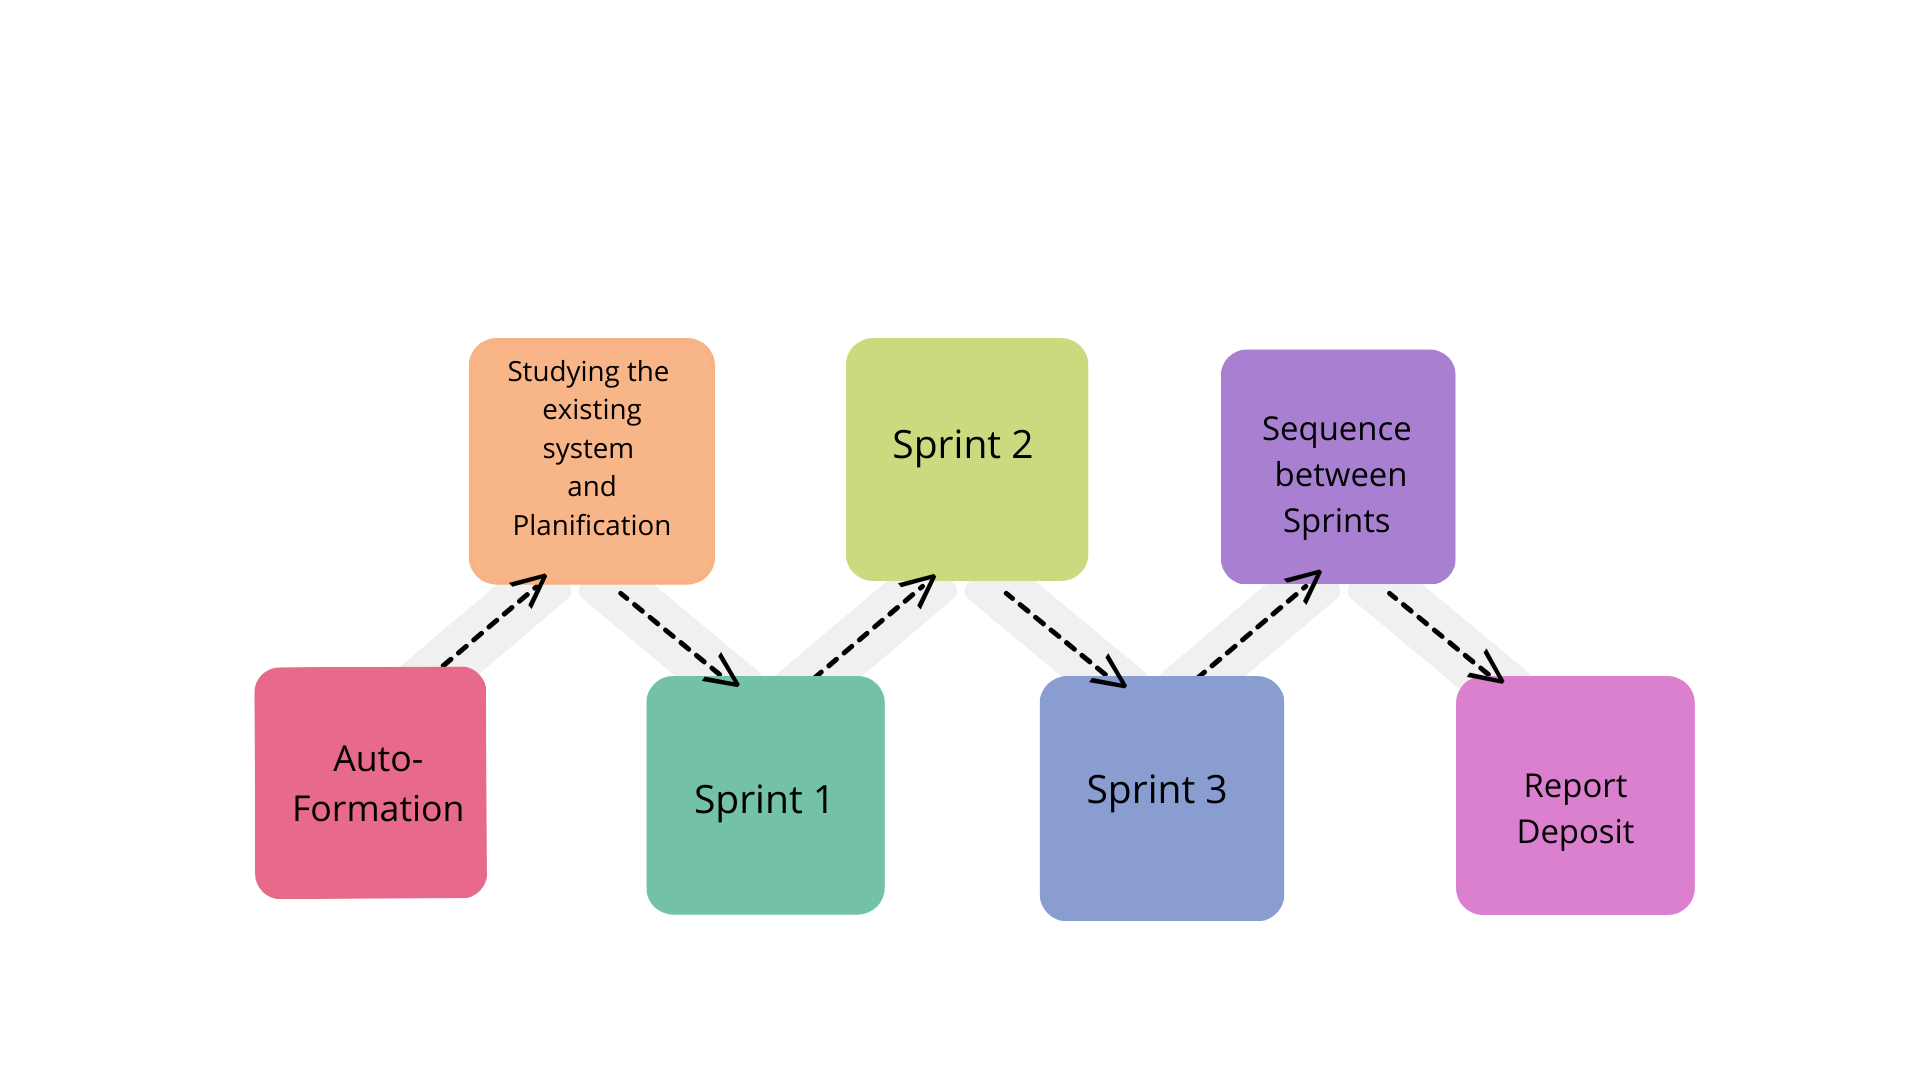
\includegraphics[width=1\textwidth]{figures/sprintplan.png} 
    \caption{Execution Plan.}
\end{figure} \
\clearpage
\begin{itemize}
    \item \textbf{15/01/2025 - 31/01/2025:} Auto-Formation.
    \item \textbf{01/02/2025 - 07/02/2025:} Studying the existing system and planification.
    \item \textbf{07/02/2025 - 28/02/2025:} Sprint 1.
    \item \textbf{01/03/2025 - 21/03/2025:} Sprint 2.
    \item \textbf{22/03/2025 - 12/04/2025:} Sprint 3.
    \item \textbf{13/04/2025 - 30/04/2025:} Sequence between Sprints.
    \item \textbf{22/05/2025}: Report deposit.
\end{itemize}
\clearpage

\section{Global Use Case Diagram}
\begin{figure}[h]
    \centering
    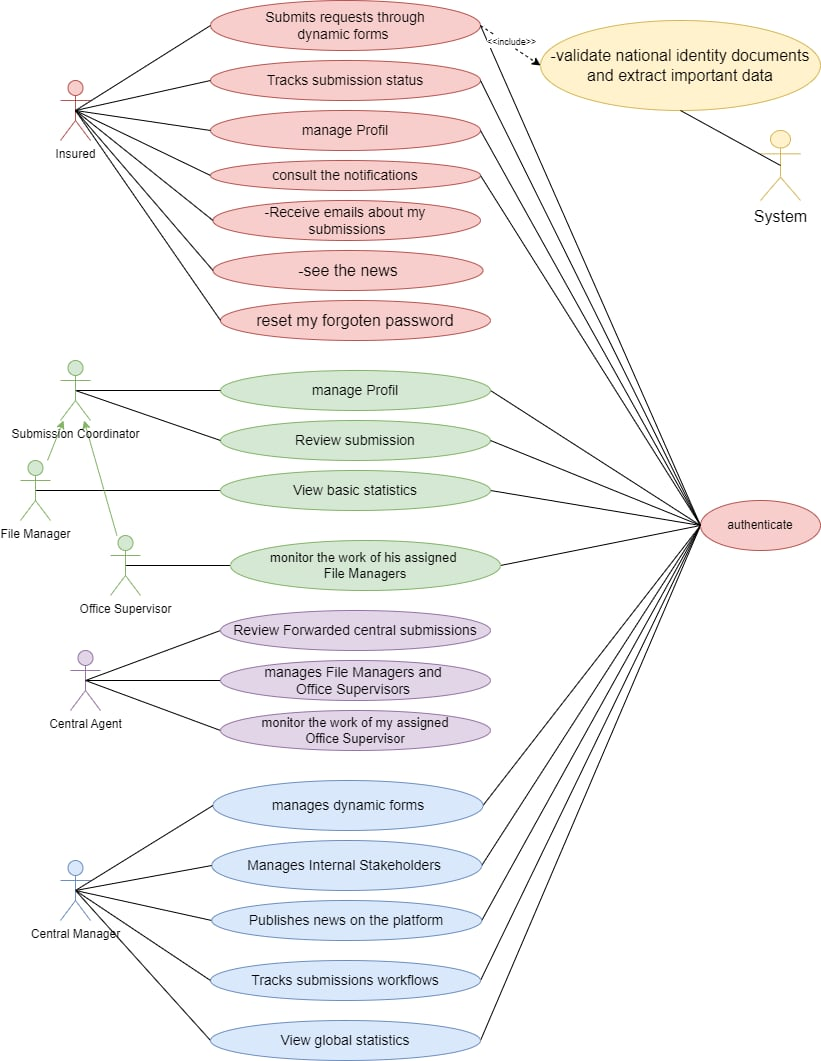
\includegraphics[width=0.9\textwidth]{figures/usecaseglobal.jpg} 
    \caption{Global Use Case Diagram.}
\end{figure} \

\clearpage
\begin{center}
    \doublespacing
    \centering
    \LARGE\textbf{Conclusion} 
    \vspace{1cm} \\
    \raggedright
\end{center}
\addcontentsline{toc}{section}{Conclusion}
In this chapter, we defined the stakeholders and outlined the product backlog based on the identification of both functional and non-functional requirements of our project.
\vspace{0.5cm}
Next, we took the first step toward Scrum by identifying the team, the product backlog, and the sprints. Finally, we created the overall use case diagram for our project.
\vspace{0.5cm}
In the next chapter, we will move on to our first sprint, which ultimately represents a potentially deliverable first version.


